\documentclass[border=3pt,tikz]{standalone}
% Shared look for every TikZ figure in these notes.
% Included by each standalone figure file; also keeps the figures consistent
% with the colours used in the PDF and on the website.

\usepackage{tikz}
\usepackage{pgfplots}
\pgfplotsset{compat=1.18}
\usetikzlibrary{arrows.meta, decorations.markings, decorations.pathmorphing,
                patterns, calc, positioning}
\usepackage{amsmath}

% Series colours are the three validated categorical slots also used by the
% interactive widgets, so a path drawn in the printed notes and the same path on
% the website are the same colour. They clear the colour-vision-deficiency and
% contrast checks as a set; every path is direct-labelled as well, so colour is
% never the only thing carrying identity.
\definecolor{duPurple}{HTML}{68246D}
\definecolor{duBlue}{HTML}{2A78D6}
\definecolor{duRed}{HTML}{EB6834}
\definecolor{duGreen}{HTML}{1BAF7A}
\definecolor{duGrey}{HTML}{4D4D4D}

\tikzset{
  % heavier default lines and arrow tips, so diagrams stay clear when zoomed
  every picture/.append style = {line width=0.7pt, >={Stealth[length=3mm]}},
  axisline/.style   = {-{Stealth[length=3.4mm]}, line width=1.0pt, black},
  path1/.style      = {duBlue,   line width=1.6pt},
  path2/.style      = {duRed,    line width=1.6pt},
  path3/.style      = {duGreen,  line width=1.6pt},
  statedot/.style   = {circle, fill=black, inner sep=1.8pt},
  arrowhead/.style  = {decoration={markings,
                        mark=at position #1 with {\arrow{Stealth[length=3.4mm]}}},
                       postaction={decorate}},
  lbl/.style        = {font=\normalsize},
  slbl/.style       = {font=\small, duGrey},
  workfill/.style   = {duPurple, opacity=0.16},
}

% larger labels in plots as well
\pgfplotsset{every axis/.append style={label style={font=\normalsize}, tick label style={font=\small}, line width=0.9pt}}

% A control volume (red dashed) with a moving boundary (piston) and a shaft
% (paddle wheel); fluid flows through along the bottom channel.
\begin{document}
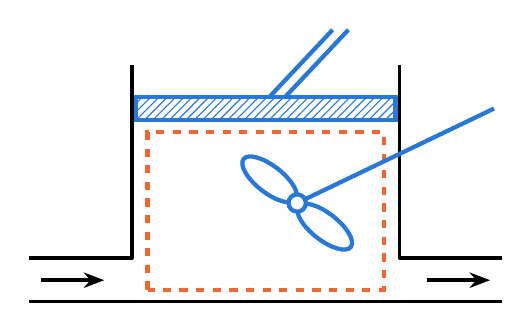
\begin{tikzpicture}[
    wall/.style={line width=1.3pt, line join=round},
    flow/.style={-{Stealth[length=2.6mm]}, line width=1.54pt}]
  % channel and walls
  \draw[wall] (-1.3,0) -- (4.7,0);
  \draw[wall] (-1.3,0.55) -- (0,0.55) -- (0,3.0);
  \draw[wall] (4.7,0.55) -- (3.4,0.55) -- (3.4,3.0);
  % piston and its rod
  \fill[white] (0.05,2.3) rectangle (3.35,2.6);
  \fill[pattern=north east lines, pattern color=duBlue] (0.05,2.3) rectangle (3.35,2.6);
  \draw[duBlue, line width=1.54pt] (0.05,2.3) rectangle (3.35,2.6);
  \draw[duBlue, line width=1.54pt] (1.75,2.6) -- (2.55,3.45);
  \draw[duBlue, line width=1.54pt] (1.95,2.6) -- (2.75,3.45);
  % control volume
  \draw[duRed, dashed, line width=1.54pt] (0.2,0.15) rectangle (3.2,2.15);
  % paddle wheel on a shaft
  \draw[duBlue, line width=1.54pt] (2.1,1.25) -- (4.6,2.45);
  \draw[duBlue, line width=1.54pt, fill=white, rotate around={-38:(1.75,1.55)}]
    (1.75,1.55) ellipse (0.42 and 0.17);
  \draw[duBlue, line width=1.54pt, fill=white, rotate around={-38:(2.45,0.95)}]
    (2.45,0.95) ellipse (0.42 and 0.17);
  \draw[duBlue, line width=1.54pt, fill=white] (2.1,1.25) circle (0.11);
  % flow in and out
  \draw[flow] (-1.15,0.27) -- (-0.35,0.27);
  \draw[flow] (3.75,0.27) -- (4.55,0.27);
\end{tikzpicture}
\end{document}
